\chapter{Arquictetura}
\label{chap:arquitetura}

\hspace{5mm} Na elaboração da arquitectura o primeiro passo foi definir as entidades em termos de classes do sistema, maior parte já detectadas no modelo de domínio. Durante esta fase o grupo apercebeu-se que fazia sentido dividir as entidades em dois grupos que se traduzem em dois subsistemas: os \textbf{Recursos Humanos} e o \textbf{Core}. Note-se que estes sub-sistemas a nível de implementação traduzem-se em dois packages.

\hspace{5mm} Os recursos humanos contém as classes que representam os utilizadores do sistema, ou seja, o cliente e personal trainer.

\hspace{5mm} No entanto após alguma pesquisa e discussão de ideias entre o grupo, percebeu-se que na actualidade as aplicações webs ou outras são orientadas a serviços.

\section{Arquitetura orientada a serviços}

\hspace{5mm} Desta forma, a ideia inicial foi separar os dois packages definidos anteriormente o \textbf{core} e os \textbf{recursos humanos}, bem como o frontend, sendo já uma boa arquitectura. No entanto, percebeu-se que que poderia ser mais bem dividido, para se tirar melhor partido, dessa forma chegou-se aos sete serviços:

\begin{itemize}
    \item Core: responsável pelas funcionalidades que interagem com planos.
    \item Requests: responsável pelas funcionalidades que interagem com os pedidos/formulários.
    \item Notifications: responsável pelas funcionalidades que interagem com as notificações.
    \item Clients: responsável pelas funcionalidades que interagem com os clientes.
    \item PersonalTrainers: responsável pelas funcionalidades que interagem com os PTs.
    \item GymAtHome: API do backend, ou seja, dispathcer dos pedidos para os serviços correctos.
\end{itemize}

\hspace{5mm} A tomada desta decisão passou por uma verificação das vantagens e desvantagens do desenvolvimento deste tipo de arquitecturas.

\hspace{5mm} As \textbf{vantagens} de desenvolver um arquitectura orientada a serviços são as seguintes:
\begin{itemize}
    \item divisão de trabalho mais fácil, aumentando assim a produtividade.
    \item divisão de responsabilidades.
    \item são mais contidos, dessa forma, mais fácil encontrar erros, bem como fazer deployment.
    \item permitem escalabilidade da arquitectura para aumento de carga.
    \item a falha de serviços não provoca directamente a falha do sistema, isto é, resiliência.
    \item quando são feitas alterações ao código, apenas necessita-se de fazer deployment do serviço alterado, não precisando de esperar por outros serviços, ou seja, deployment contínuo.
    \item permitem mais flexibilidade da arquitectura.
    \item ...
\end{itemize}

\hspace{5mm} As \textbf{desvantagens/falácias} cometidas quando de desenvolve orientado a serviços:
\begin{itemize}
    \item pensar que a banda larga é infinita.
    \item pensar que não existe latência.
    \item pensar que os dispositivos de rede são uniformes.
    \item pensar que não existem hackers.
    \item necessidade de mais recursos.
    \item ...
\end{itemize}

\hspace{5mm} No entanto, apesar de conter-se algumas desvantagens, as vantagens sobrepõem-se, obtendo-se melhores resultados a nível de escalabilidade com uma arquitectura orientada a serviços.

\hspace{5mm} Na verdade, "nem tudo é um mar de rosas", ao desenvolver uma arquitectura orientada a serviços, acresce uma complexidade, que consiste em manter serviços consistentes, pois alguns depende dos dados de outros, como por exemplos os outros serviços dependem do clientes e personal trainers, pois quando existe o registo dos mesmos, tem-se que propagar essa \textbf{escrita} para todos os serviços. No entanto, mais uma vez, esta complexidade extra em alguns serviços, não sobrepõe as vantagens.

\hspace{5mm} Outro problema encontrado nesta arquitectura foi a necessidade mais recursos de CPU e RAM do que o costume. No entanto em produção não seria problema, visto que seriam disponibilizados mais recursos. 

\hspace{5mm} De seguida, serão apresentadas as várias decisões, tomadas na arquitectura, bem como a apresentação dos serviços individualmente.

\section{Client Service}

\hspace{5mm} O package HRClient (HR alusivo a Human Resource) encontra-se especificado nas seguintes figuras.

\begin{figure}[H]
    \centering
    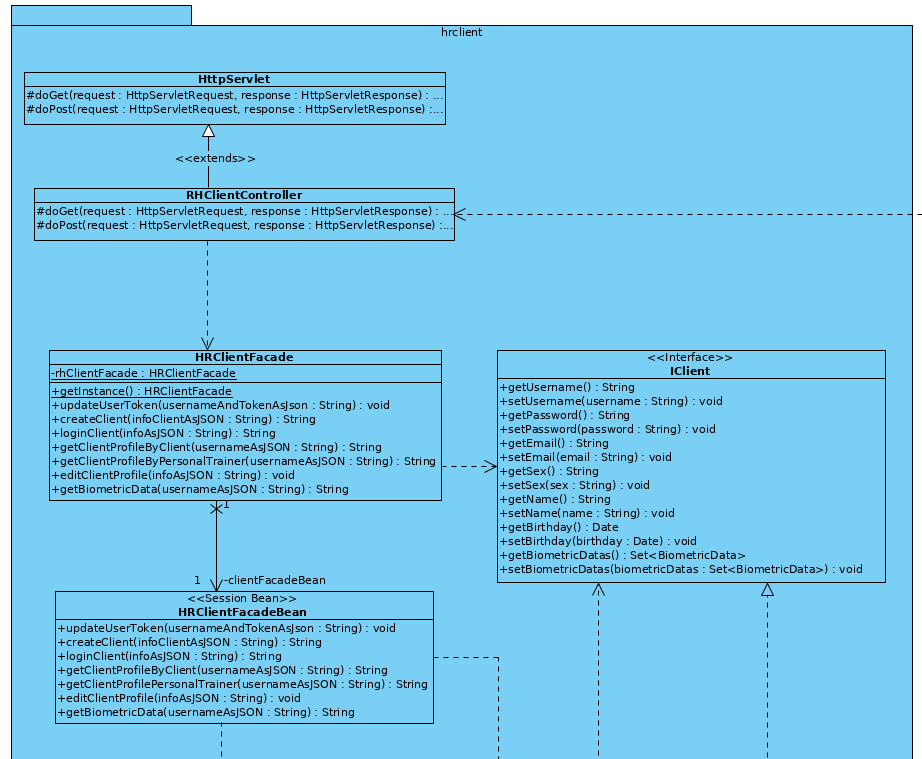
\includegraphics[scale=0.575]{images/arquitetura/client-package-1.png}
    \caption{Diagrama de classes do package HRClient - parte 1.}
    \label{fig:interfaceperfilptbycliente}
\end{figure}


\begin{figure}[H]
    \centering
    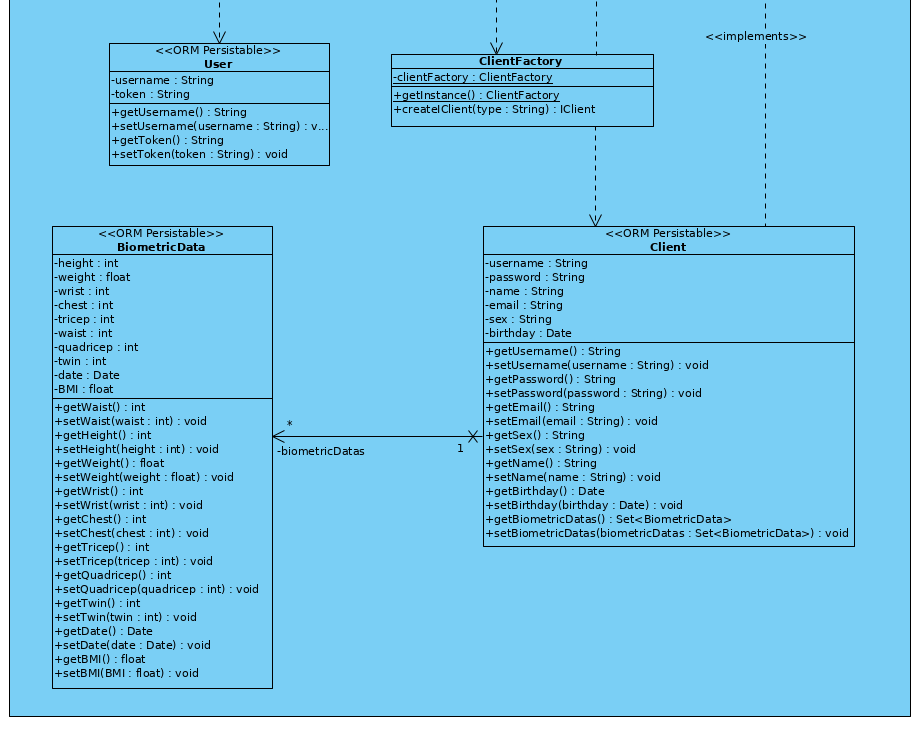
\includegraphics[scale=0.575]{images/arquitetura/client-package-2.png}
    \caption{Diagrama de classes do package HRClient - parte 2.}
    \label{fig:interfaceperfilptbycliente}
\end{figure}


\hspace{5mm} Em relação ao cliente foi criada a classe \textbf{Client} com a informação específica do mesmo, tal como referido anteriormente no modelo de domínio, o cliente contém um histórico de dados biométricos, para isso foi criada uma associação entre a classe Client e a classe \textbf{BiometricData}. \textbf{Note-se que a relação é de um para muitos uma vez que existe a noção de histórico} apesar de não estar implementada a funcionalidade de visualização do mesmo a na UI. De seguida foi introduzida a interface \textbf{IClient} de forma a que as classes que utilizam a mesma \textbf{dependam apenas da interface e não da classe concreta}. Esta prática \textbf{facilita a evolução e manutenção do código} pois caso, no futuro, sejam introduzidas novas classes concretas que representam clientes (ex: ClientPremium, etc) desde que as mesmas implementem o tipo IClient, o código continuará a funcionar sem alterações. 

\subsection{Factory Method}

\hspace{5mm} Com o mesmo objectivo, para facilitar a evolução e manutenção do código, foi introduzido o \href{https://refactoring.guru/design-patterns/what-is-pattern}{design pattern} \href{https://refactoring.guru/design-patterns/factory-method}{Factory Method} que é responsável pela criação dos clientes. Para tal foi criada a classe \textbf{Factory Method}. A grande vantagem da utilização deste design pattern é que o processo de criação/ instanciação do objecto do tipo IClient passa a ser responsabilidade da classe ClientFactory, desta forma as classes que utilizam o IClient em vez de dependerem dos tipos concretos (uma vez que antes as próprias faziam a instanciação do objecto) passam a depender apenas da interface IClient e da classe ClientFactory. \textbf{Analisando a arquitectura actual, pode parecer que não houve vantagem na introdução do Factory Method uma vez que antes existiam 2 dependências, com a interface IClient e a classe Client e após a introdução do mesmo continuam a existir o mesmo número de dependências, neste caso com a interface IClient e classe ClientFactory. No entanto, numa perspectiva evolutiva e pensando no futuro, caso sejam introduzidas N classes do tipo IClient, as dependências são reduzidas de N+1 (N classes + interface IClient) para 2 apenas (ClientFactory + IClient)} por este motivo o grupo entendeu que se justifica a introdução do Factory Method.

\hspace{5mm} Note-se que apesar do design pattern referido anteriormente ter sido introduzido na proposta inicial da arquitectura, após gerado o código, na prática acabou por não ter sido implementado pelo grupo uma vez que foi utilizada a API \href{https://github.com/google/gson}{gson}, desenvolvida pela Google, responsável pela serialização e deserialização de objectos Java para o formato \href{https://en.wikipedia.org/wiki/JSON}{JSON}. Esta API internamente já implementa o Factory Method por isso não foi necessário uma implementação concreta pelo grupo. No entanto a classe ClientFactory permanece no código, apesar de não implementada, para que, caso, no futuro, seja necessária a sua utilização, a arquitectura já conte com a mesma. Para clarificar, uma possível hipótese de necessidade de utilizar a própria implementação por parte do grupo seria por exemplo, caso a API gson fosse descontinuada. 

\subsection{Adpater}

Ainda devido à utilização da API referida anteriormente foi necessária a introdução do design pattern \href{https://refactoring.guru/design-patterns/adapter}{Adapter} uma vez que a API apenas consegue serializar/deserializar certos tipos de objectos conhecidos (int, boolean, String, List, Array, Date, etc) por isso para serializar/deserializar um Client visto que tem uma relação com a classe BiometricData é necessário indicar como essa serialização/deserialização deve ser feita, sendo a mesma através de classes auxiliares como a \textbf{BiometricDataSerializer} que se comporta como um adaptador do tipo BiometricData.

\subsection{Hibernate}

\hspace{5mm} Tanto as classes User (mais á frente explicada), Client como BiometricData foram identificadas como \textbf{ORM Persistable} uma vez que se pretende persistir a informação das mesmas. Para tal utilizou-se a framework \href{https://hibernate.org/}{Hibernate} integrada como plugin (built-in) na ferramenta \href{https://www.visual-paradigm.com/}{Visual Paradigm} de modo a automatizar a criação das classes \href{https://www.tutorialspoint.com/design_pattern/data_access_object_pattern.htm}{DAO} que são responsáveis por realizar operações CRUD  (entre outras interrogações) sobre os objectos persistidos. Para tal a framework hiberante fornece \textbf{mapeamento automático (ou de fácil configuração) das classes (neste caso Java) para tabelas numa base de dados relacional} (neste caso MySQL) através da sinalização no diagrama de classes ou anotações no código gerado. Ainda fornece \textbf{abstracção da tecnologia de conexão à base de dados, inclusive gestão de sessões}, podendo, por isso, ser configurada para diferentes base de dados, \textbf{sem alteração do código}. No entanto tem a desvantagem de existir um acréscimo computacional no uso da framework, ainda assim analisando as vantagens oferecidas compensa a utilização da mesma.

\subsection{EJB}

\hspace{5mm} Foi criada também a classe \textbf{HRClientFacadeBean} que implementa uma \textbf{Session Bean Stateless} onde as operações a realizar são definidas. A utilização dos EJB fornece a gestão automática de \textbf{sincronização das interacções entre objectos em ambiente concorrente}, gestão da \textbf{partilha de recursos/ objectos entre componentes ou intervenientes no sistema}, por exemplo na partilha das sessões na conexão à base de dados, utiliza a \textbf{JNDI} que é uma API de lookup que permite a \textbf{procura de recursos (procura da referência do recurso) através de um nome previamente atribuído a esse mesmo recurso}, fornece também \textbf{interoperabilidade}, por exemplo através de protocolos como o \textbf{WSDL}, apesar do grupo não ter utilizado neste projecto, uma vez que foi utilizado o protocolo \textbf{REST} para comunicação entre serviços que será detalhado mais à frente, a utilização de EJBs disponibiliza outras funcionalidades não referidas. Em suma, o grupo entendeu que a utilização de EJBs é vantajosa uma vez se adequa ao contexto de utilização do sistema pois existem:

\begin{itemize}
    \item muitos utilizadores, isto é, muitas instâncias de aplicações cliente;
    \item milhares de objectos criados e em utilização;
    \item muitas interacções entre os objectos;
    \item concorrência e operações com requisitos transaccionais.
\end{itemize}

\subsection{Multi-camada e Facade}

\hspace{5mm} De forma a implementar o \href{https://en.wikipedia.org/wiki/Architectural_pattern#:~:text=An\%20architectural\%20pattern\%20is\%20a,minimization\%20of\%20a\%20business\%20risk.}{padrão arquitectural} denominado por \href{https://en.wikipedia.org/wiki/Multitier_architecture}{multi camada} foi implementado o design pattern \href{https://refactoring.guru/design-patterns/facade}{Facade} que expõe a \textbf{API} do serviço contido nesse package de modo a que \textbf{as classes contidas nos packages exteriores apenas comuniquem com as classes internas a este package através de um único ponto}, neste caso a classe \textbf{HRClientFacade}, reduzindo assim o número de dependências entre os packages. Para se entender a vantagem deste design pattern, segue-se um exemplo: caso o package business apenas comunique com o package data através do DataFacade, se a implementação interna do package data muda-se drasticamente, \textbf{o package business não sofria qualquer alteração} desde que a classe DataFacade continuasse a existir e mantive-se os protótipos dos seus métodos inalterados, isto é, a sua API inalterada.

\subsection{Singleton}

\hspace{5mm} Ainda neste package, visto que ambas as classes ClientFactory e HRClientFacade devem ter um única instância em todo o sistema foi implementado o design pattern \href{https://refactoring.guru/design-patterns/singleton}{Singleton}.

\subsection{REST vs WSDL}

\hspace{5mm} De forma a tornar a funcionalidade fornecida por este package \textbf{facilmente acessível por qualquer outro serviço ou sistema} foi implementado um servidor utilizando Java Servlets contidos na API Java EE, na qual a classe que implementa o Servlet, neste caso denominada por \textbf{HRClientController}, responde a pedidos recebidos através do protocolo \textbf{HTTP}. O grupo decidiu utilizar o protocolo REST ao invés de WSDL para a comunicação entre serviços uma vez que a complexidade de cada serviço é relativamente reduzida (consequência directa da divisão do sistema em serviços menos complexos), outra razão é o facto de existir total conhecimento no contexto de utilização e conteúdo transmitido nos pedidos HTTP, por 
último visto que na componente frontend, algumas funcionalidades são acedidas por \textbf{AJAX}, a utilização de REST torna-se mais adequada. 


\subsection{Token Authentication}

\hspace{5mm} Observando o diagrama de classes deste package existe uma classe ainda não abordada, a classe \textbf{User}. Esta classe foi criada unicamente para implementar um método de autenticação do utilizador, quer seja um cliente ou personal trainer, na evocação externa de qualquer método. Desta forma no momento de \textbf{registo} ou \textbf{login} de qualquer utilizador no sistema é gerado um \textbf{token único e aleatório} armazenado no sistema numa instância da classe User e retornado ao utilizador para que seja também armazenado temporariamente na aplicação client-side, assim numa futura evocação de qualquer método o token é verificado e caso coincide é permitida a interacção do utilizador.


\section{Personal Trainer Service}

\hspace{5mm} O package HRPersonalTrainer encontra-se especificado nas seguintes figuras.

\begin{figure}[H]
    \centering
    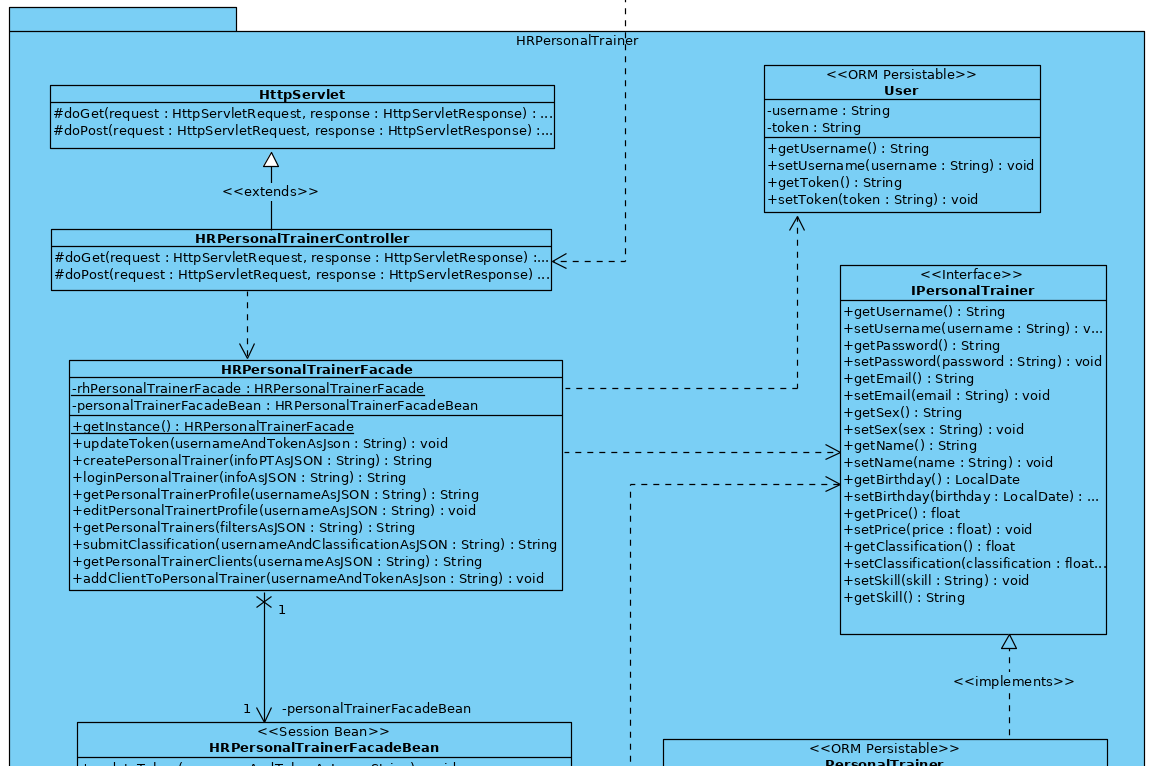
\includegraphics[scale=0.45]{images/arquitetura/pt-package-1.png}
    \caption{Diagrama de classes do package HRPersonalTrainer - parte 1.}
    \label{fig:interfaceperfilptbycliente}
\end{figure}


\begin{figure}[H]
    \centering
    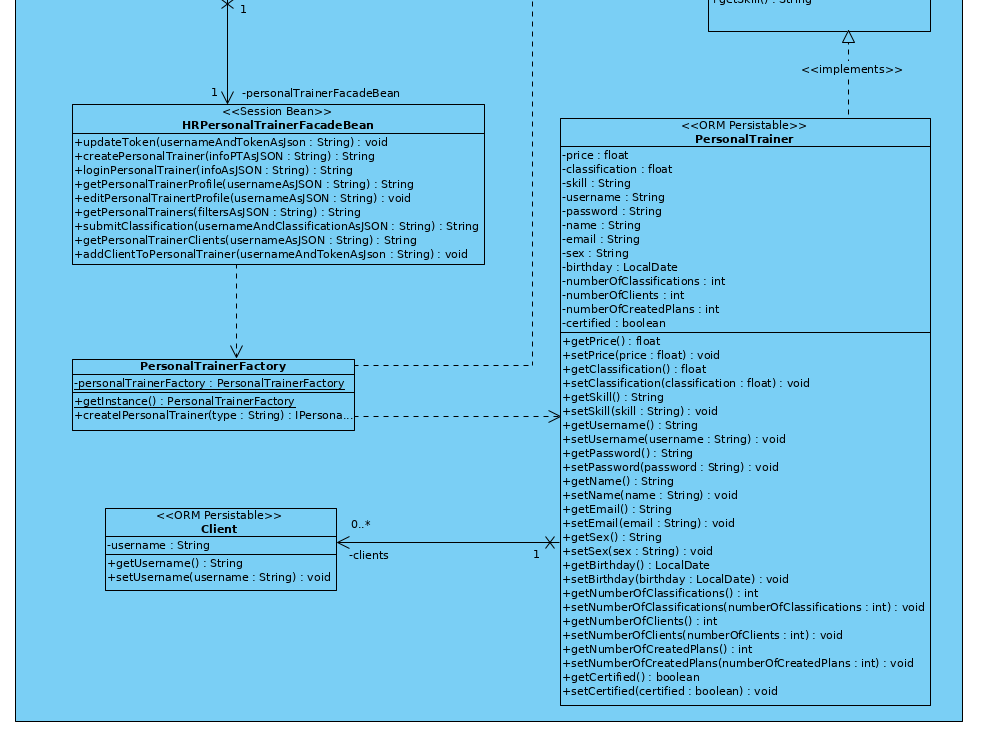
\includegraphics[scale=0.5]{images/arquitetura/pt-package-2.png}
    \caption{Diagrama de classes do package HRPersonalTrainer - parte 2.}
    \label{fig:interfaceperfilptbycliente}
\end{figure}

\hspace{5mm} Analogamente ao Client Service e pelos mesmos motivos no package HRPersonalTrainer foram implementados os design pattern: \textbf{FactoryMethod, Adapter, Singleton e Facade}. A lógica de negócios foi, também, implementada num \textbf{Session Bean} e o serviço exposto através do protocolo \textbf{REST} utilizando \textbf{autenticação por tokens}.

\hspace{5mm} No entanto foi necessária a associação entre um cliente e um personal trainer para isso foi introduzida a classe \textbf{Client} também esta persistida.

\section{Core}

\hspace{5mm} O package Core encontra-se especificado nas seguintes figuras.

\begin{figure}[H]
    \centering
    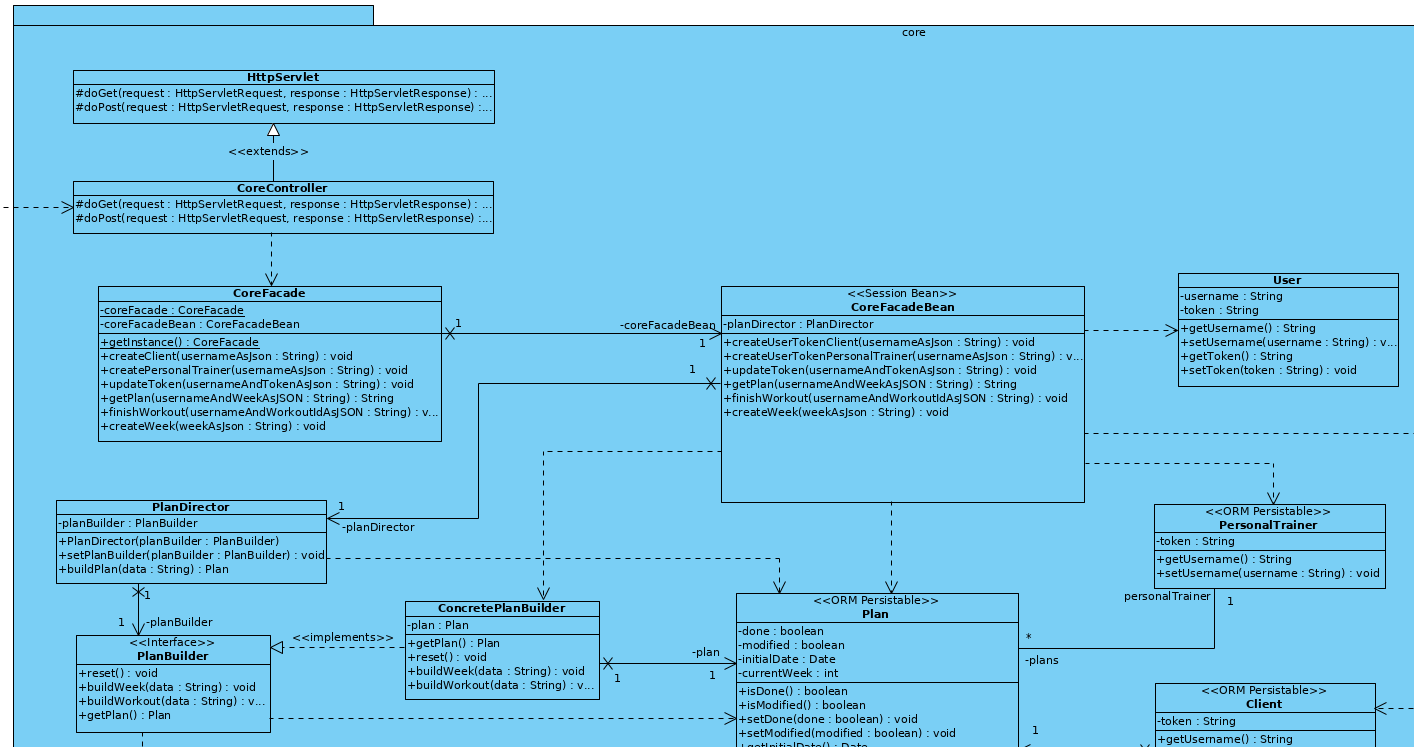
\includegraphics[scale=0.35]{images/arquitetura/core-package-1.png}
    \caption{Diagrama de classes do package Core - parte 1.}
    \label{fig:interfaceperfilptbycliente}
\end{figure}


\begin{figure}[H]
    \centering
    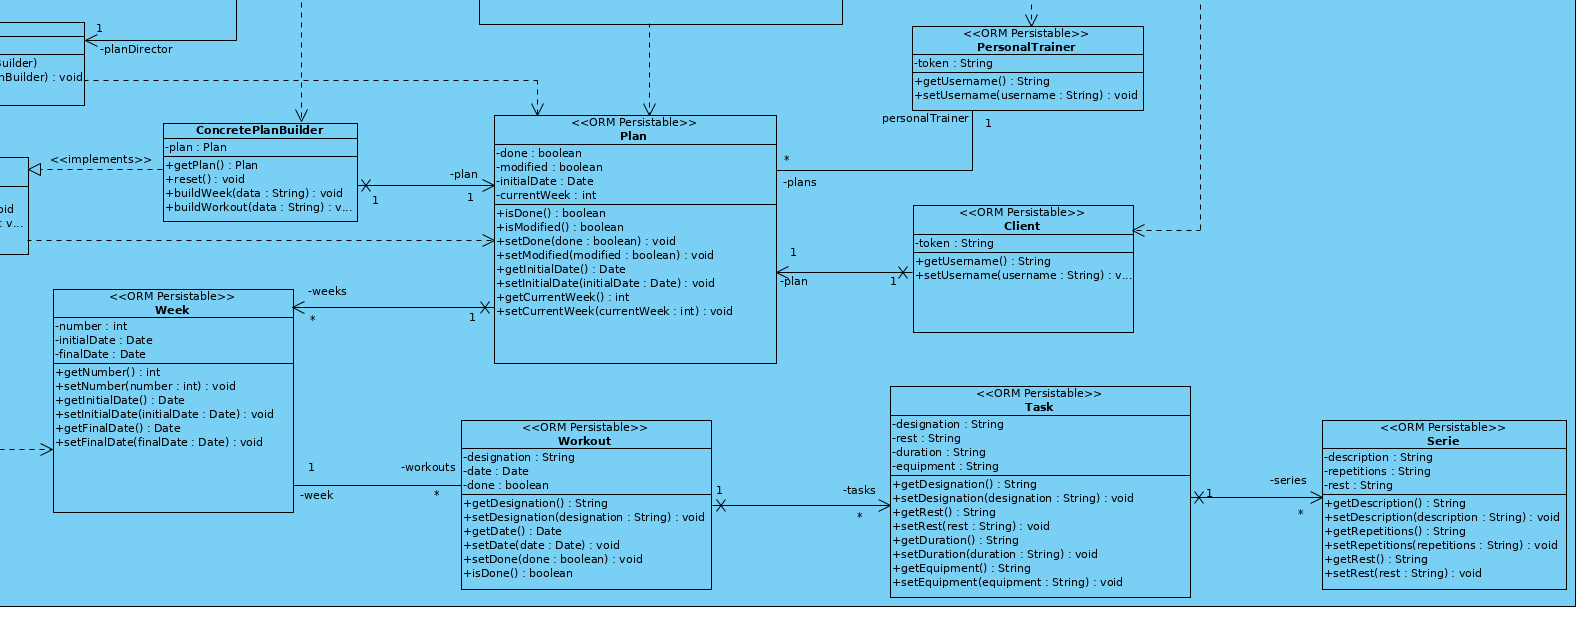
\includegraphics[scale=0.325]{images/arquitetura/core-package-2.png}
    \caption{Diagrama de classes do package Core - parte 2.}
    \label{fig:interfaceperfilptbycliente}
\end{figure}

\hspace{5mm} O Core contém as entidades principais do modelo de negócio, no contexto deste projecto, contém as classes: \textbf{Plan}, \textbf{Week}, \textbf{Workout}, \textbf{Task} e \textbf{Serie}; já descritas anteriormente no modelo de domínio.

\hspace{5mm} Analogamente aos serviços anteriores e pelos mesmos motivos no package Core foram implementados os design pattern: \textbf{Adapter, Singleton e Facade}. A lógica de negócios foi, também, implementada num \textbf{Session Bean} e o serviço exposto através do protocolo \textbf{REST} utilizando \textbf{autenticação por tokens}.

\hspace{5mm} Note-se na relação entre certas classes foi vantajoso utilizar a dupla navegabilidade uma vez que o dupla direcção no acesso entre ambos os objectos é útil. 

\subsection{Método finishWorkout}

\hspace{5mm} O método \textbf{finishWorkout()} responsável por finalizar um determinado Workout tem elevada relevância no sistema. Não só realiza a operação evidente de Update (neste caso actulização do estado do workout para realizado), mas também tem uma funcionalidade adicional tal como, avançar automaticamente a semana do plano em que o cliente se encontra caso todos os workouts dessa semana tenham sido realizados. Para clarificar segue-se um exemplo, caso por exemplo o Plano de treino do Cliente se encontre na semana 3 (semana actual), mas se este realizar todos os workouts da semana 5 a sua semana actual passa a ser a 6, este sistema de actualização da semana actual foi baseado em outras aplicações, tal como a Netflix, em que se um utilizador estiver na temporada 3, mas depois for ver um episódio da temporada 5, quando voltar a entre no site para voltar a ver a série será remetido automaticamente para a temporada 5.

\subsection{Builder}

\hspace{5mm} No Core foi implementado o Design Pattern Builder, este é um Pattern criacional, no qual os principais objectivos é reduzir o número de dependências, pois todos as classes apenas ficam dependentes do PlanDirector, sendo este o único a ter as dependências necessárias. Outro objectivo é a criação do objecto por passos.

\hspace{5mm} Tal como nos serviços Client e PT o este design pattern acabou por não ser implementado em código porque a biblioteca GSON consegue ela própria criar o objecto todo através de um json e das classes de Deserialização criadas.

\section{Requests Service}

\hspace{5mm} Analogamente ao serviços anteriores e pelos mesmos motivos no package Requests foram implementados os design pattern: \textbf{Singleton e Facade}. A lógica de negócios foi, também, implementada num \textbf{Session Bean} e o serviço exposto através do protocolo \textbf{REST} utilizando \textbf{autenticação por tokens}.

\hspace{5mm} O serviço Requests tal como o nome sugere é um serviço que guarda informações sobre pedidos, pedidos estes submetidos por Clientes para os PTs, nos quais consta informação sobre o tipo de Plano que desejam realizar. O Cliente tem acesso a todos os pedidos que realizou, por outro lado o PT só tem acesso aos pedidos que ainda tem pendentes.

\hspace{5mm} Os Pts podem aceitar ou rejeitar pedidos sempre essa informação ilustrada aos Clientes, pois o aceitar ou rejeitar de um pedido altera o seu estado.

\begin{figure}[H]
    \centering
    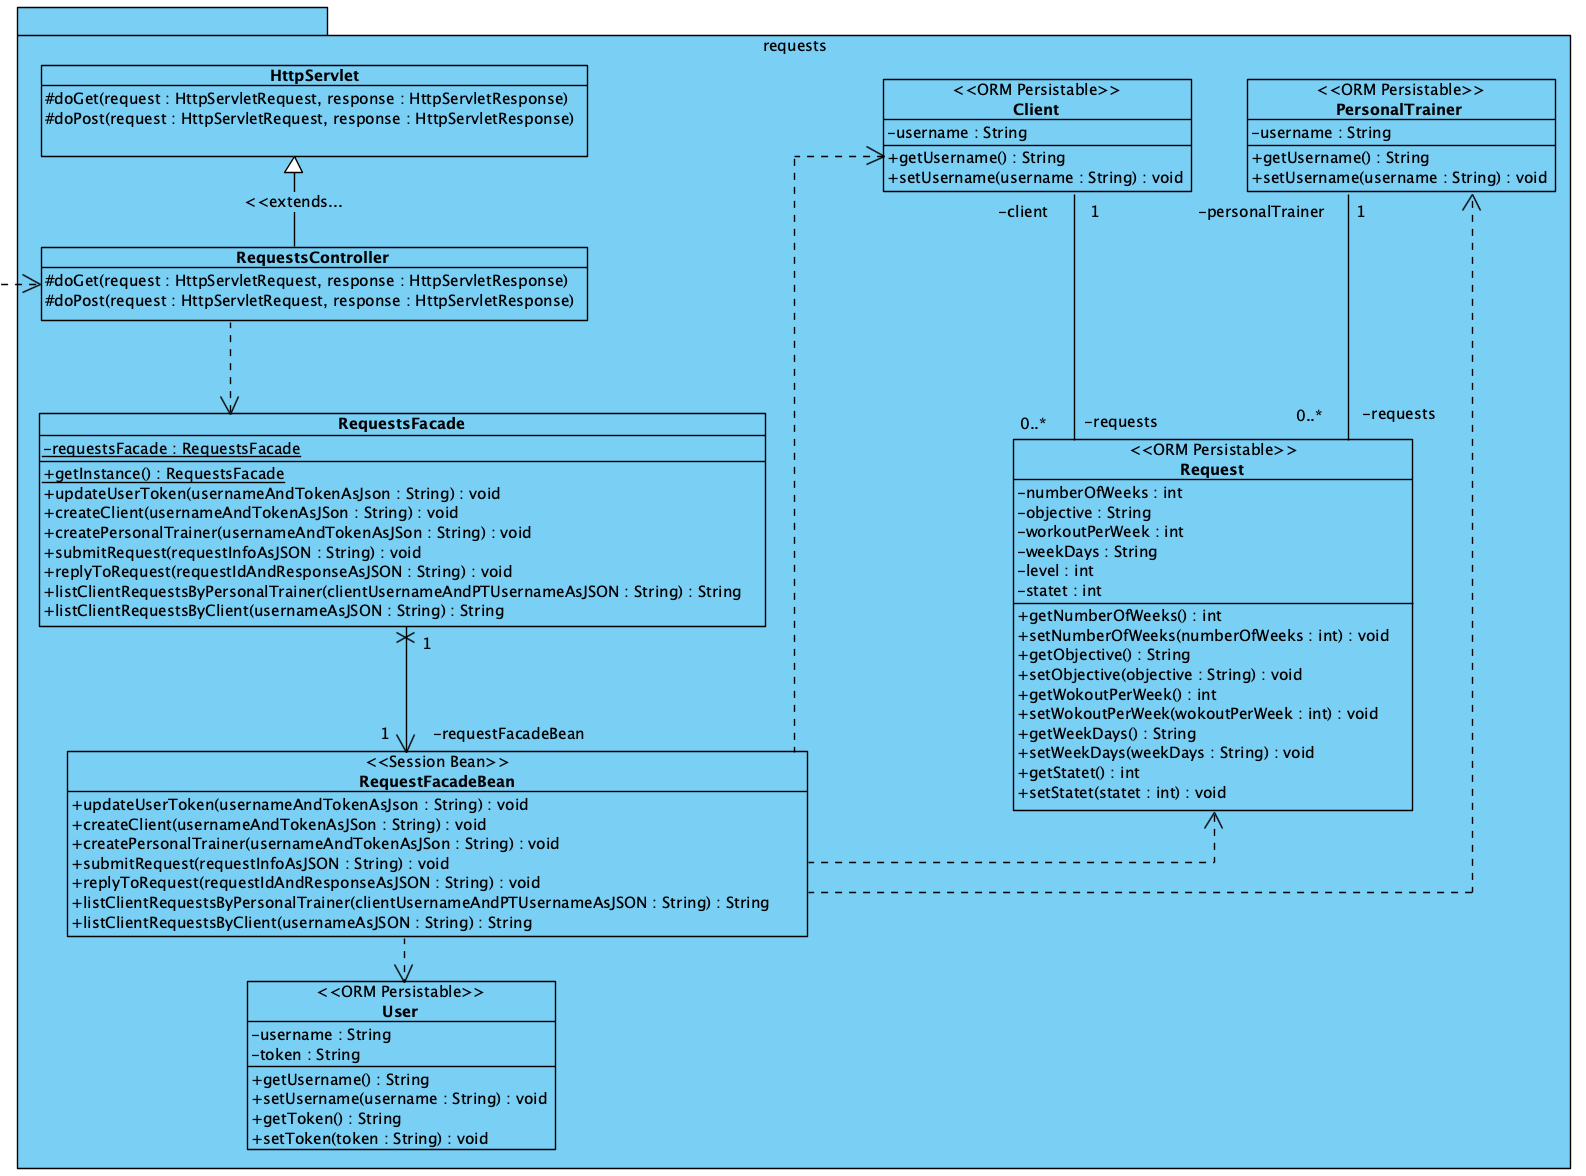
\includegraphics[scale=0.5]{images/arquitetura/requests-package.png}
    \caption{Diagrama de classes do package Notification}
    \label{fig:my_label}
\end{figure}

\section{Notifications Service}

\hspace{5mm} Analogamente ao serviços anteriores e pelos mesmos motivos no package Notifications foram implementados os design pattern: \textbf{Singleton e Facade}. A lógica de negócios foi, também, implementada num \textbf{Session Bean} e o serviço exposto através do protocolo \textbf{REST} utilizando \textbf{autenticação por tokens}.

\hspace{5mm} O serviço Notifications tal como o nome sugere é um serviço que guarda as notificações geradas pelo sistema para os utilizadores. O sistema apenas gera notificações consoante acções de utilizadores, estes quando realizam uma acção relacionada com outro o sistema irá criar uma notificação para o outro utilizador, de forma a que esta possa ser informado de alterações que existiram no sistema.

\hspace{5mm} Tanto os Clientes como os PTs podem marcar as notificações como lidas, desta forma será mais fácil numa próxima vista das notificações distinguir daquelas que estão por ler e as que já estão lidas.

\begin{figure}[H]
    \centering
    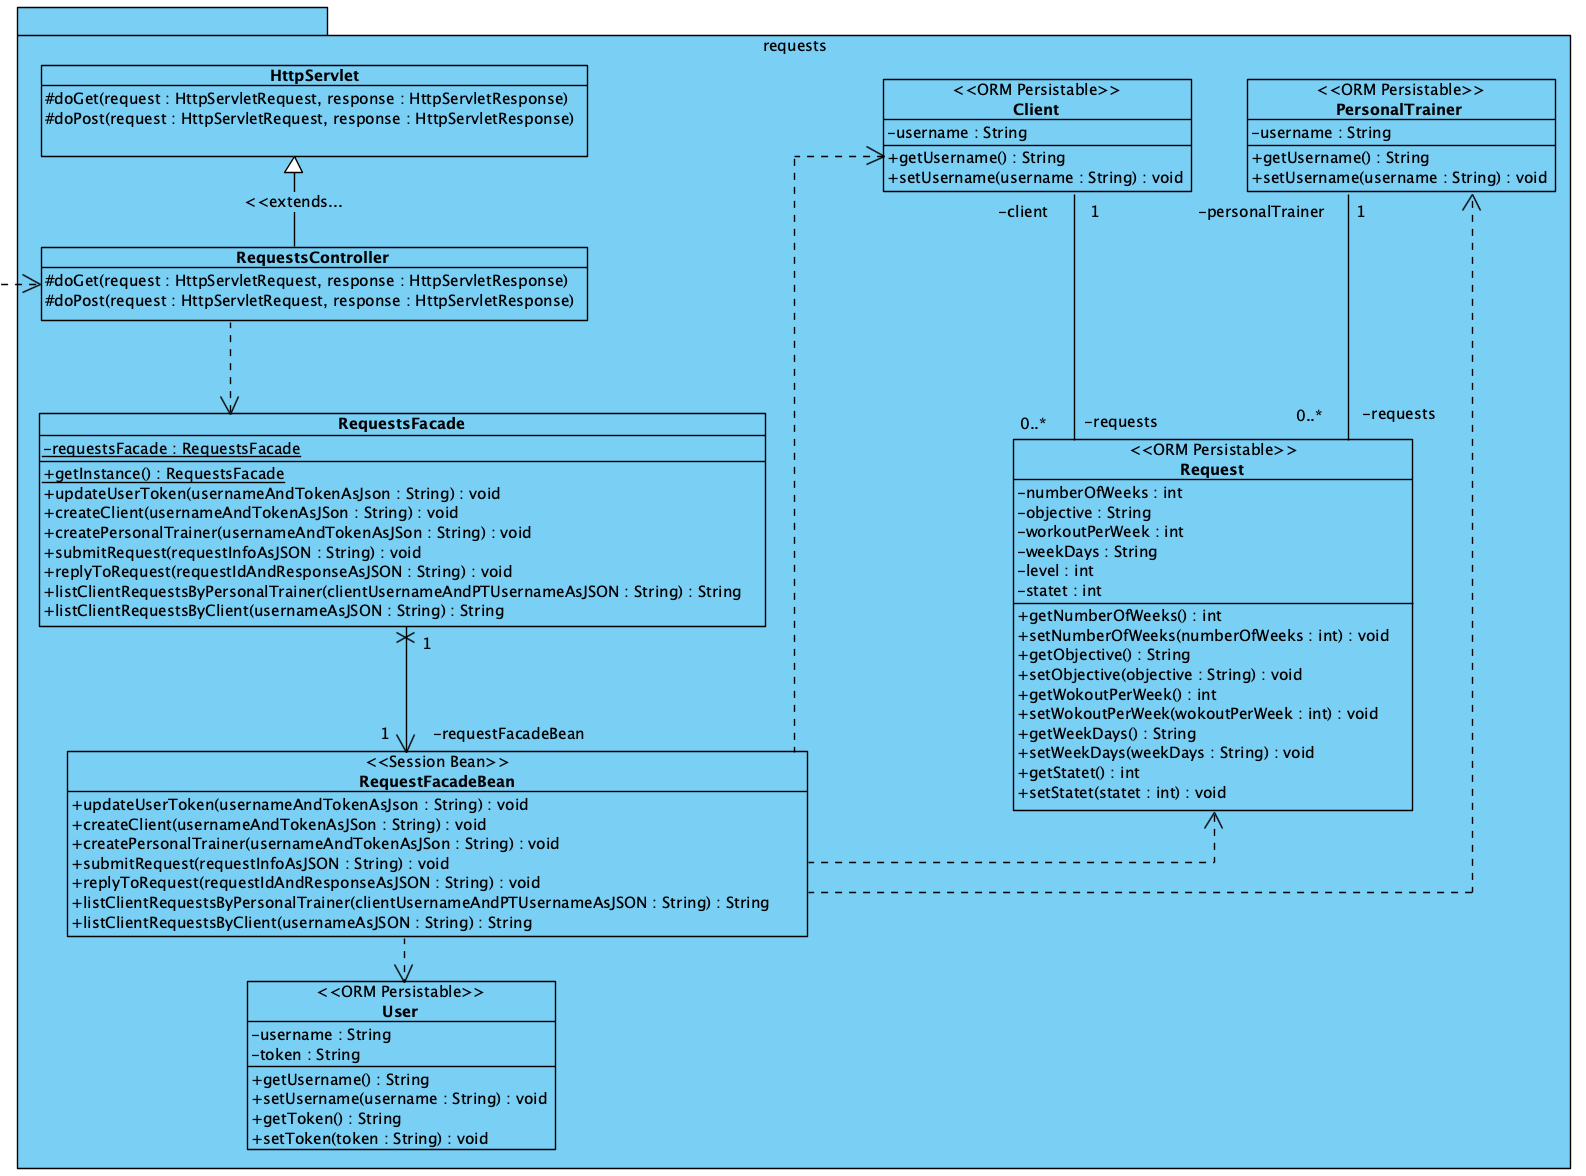
\includegraphics[scale=0.5]{images/arquitetura/requests-package.png}
    \caption{Diagrama de classes do package Request}
    \label{fig:my_label}
\end{figure}

\section{GymAtHome Service}

\subsection{Propagação dos tokens}

\hspace{5mm} Tal como referido anteriormente todos os serviços contêm um método de autenticação da interacção do utilizador através de um token gerado no login ou registo. Desta forma para que todos os serviços tenham todos os tokens mais actuais de cada cliente, este serviço principal (GymAtHome) tem a responsabilidade de propagar os tokens para os respectivos serviços externos, para isso foi definido o método updateToken nos mesmos.

\hspace{5mm} Este serviço serviço tem ainda o objectivo de criar notificações para os utilizadores, à medida que os utilizadores realizam certas acções podem ser geradas algumas notificações.

\hspace{5mm} A principal função deste serviço é servir de dispatcher, pois todos os pedidos enviados pelo \href{sec:frontend}{Frontend} são direccionados a este e este é que trata de encaminhar para o serviço correcto e de apenas reencaminhar a resposta do serviço que comunicou. Com os isto os outros serviços estão mais protegidos uma vez que o único ponto de acesso destes é através deste serviço.

\section{Frontend service}
\label{sec:frontend}

\subsection{MVC - Model View Controller}

\hspace{5mm} Para a comunicação entre os \textbf{Controllers} e respectivas páginas de apresentação (\textbf{Views}) foi implementado o padrão arquitectural \href{https://en.wikipedia.org/wiki/Model\%E2\%80\%93view\%E2\%80\%93controller}{MVC}. O acesso ao \textbf{Model} (que contem a lógica de negócio), por parte do Controller é realizado através do protocolo REST. A utilização deste padrão arquitectural, novamente, torna a evolução e manutenção do código facilitada uma vez que, por exemplo, caso o pacakage presentation (que contém os Controllers e respectivas Views) seja alterado, por exemplo, ao implementar uma nova UI para o sistema operativo Android ou IOS, visto que toda a lógica de negócio está unicamente contida no Model, o sistema (na componente backend) continuará totalmente funcional e inalterado.